% !TEX root = mythesis.tex

%==============================================================================
\chapter{Conclusion and Outlook}
\label{chap:conc}
%==============================================================================
% \begin{figure}[h!]
% \centering
% 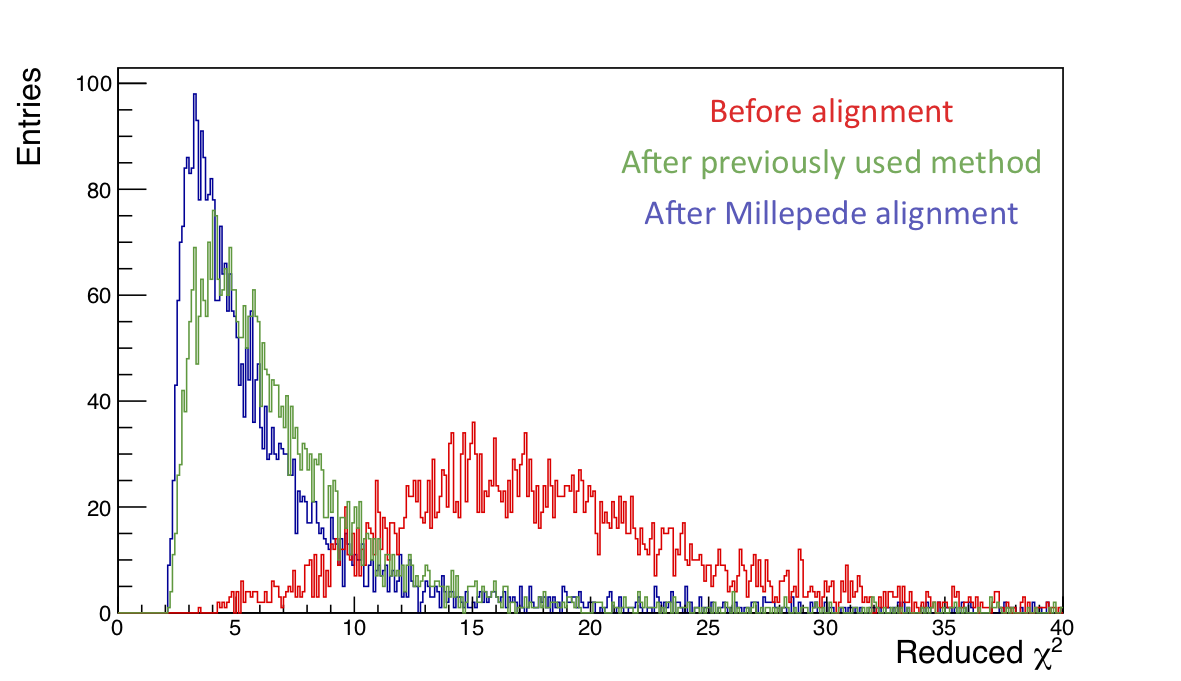
\includegraphics[width=0.85\textwidth]{thesis_figures/chi2_comp_conclusion_2.png}
% \caption{$\chi^2_{red}$ distribution for selected tracks showing the impact of Millepede alignment.}
% \label{fig:red_chi2_4}
% \end{figure}

Besides detecting ultra-high-energy (UHE) cosmic rays, the Pierre Auger Observatory with its large Surface Detector (SD) array offers a remarkable exposure to neutrinos above $10^{17}$eV. Any potential observation of such UHE$\nu_s$ will further our knowledge about the known universe. Since neutrinos are not deflected as they travel towards us at Earth, they offer a direct line of sight to the sources where they were produced. They are also some of the earliest particles produced in a transient source which makes their detection an important beacon for other astronomical instruments to perform a multi-messenger observation. The Pierre Auger Observatory is constantly monitoring the sky for the presence of such UHE$\nu_s$. The idea behind the detection remains the same as previous analysis at Auger where the neutrinos are assumed to induce Extensive Air Showers (EASs) close to the ground with a large electro-magnetic component at ground ("young" showers). This strategy is only employed for horizontal showers ($\theta > 60^{\circ}$). Two new SD triggers, time-over-threshold-deconvolved (ToTd) and multiplicity of positive steps (MoPS) were installed in 2014 to further increase the detection efficiency for low energy neutrino induced EASs. This thesis presents the first analysis of this improved efficiency for low energy neutrino showers in the zenith range $\theta \in [60^{\circ},75^\circ]$ also known as Down-going low or DG$_{Low}$ range. In this thesis the effect of the new triggers was evaluated for two types of searches, the searches for the diffused flux of UHE$\nu_s$ and search for point-like sources of UHE$\nu_s$. For both searches an overall improvement of efficiency is observed when information from the new triggers is incorporated in the analysis. A short summary of the three main contributions of this thesis along with an outlook detailing potential improvements are detailed in the next sections. 
\section*{Incorporating new triggers in the DG$\mathrm{_{low}}$ UHE$\nu_s$ searches}
During this thesis each facet of the DG$_{low}$ analysis was analysed. An effort was made to maximize the potential of the analysis. A blind search strategy similar to~\cite{gap_note_2013,Aab_2019_diffuse} was followed to avoid any bias in the analysis. The first step in this process was to include the information from the new triggers in the neutrino searches. About $\sim$7 years of recorded data was available for this task. The effect of the new triggers was first evaluated on neutrino simulations by including them in the analysis chain as described in section~\ref{subsubsec:nu_sel_fisher_training}. By the inclusion of new triggers an overall increase in reconstructed events was observed as shown in fig~\ref{fig:Events_vs_angle_summary}. This increase was most significant for lower energy neutrinos and decreased with increase in primary energy. This was an expected consequence due to the design of the new triggers. The overall increase also allowed for further modifications to the analysis which included lowering some stringent cuts as described in section~\ref{subsec:nu_sel_nudeteff}. For the final step of the analysis a Fisher discriminate polynomial was built and trained using the simulations (signal training sample) and a small fraction of recorded data, $\sim$20\% from the Observatory (background training sample). The polynomial is built with Area over Peaks (AoPs) of the stations and a differentiation between the background and signal is performed based on a cut on the Fisher value as given in eq.~\ref{eq:fisher_poly_cut}.
After the fixing the selection, a test sample was unblinded to catch any remaining flaws in the analysis. This proved worthwhile as a small error in the reconstruction was discovered during this process. The error was promptly corrected, and the whole selection procedure was re-evaluated, and the Fisher was retrained. Since the correction involved a change to the reconstruction procedure the blind search was redone from the start. After this correction the unblinding was again performed in two stages. The new test sample and the full blinded sample, 20\% + 60\% of recorded data between the period of 1 Jan 2014 to 31 December 2012 was analysed to search for neutrinos. \textbf{No neutrino candidates} were found in the search performed using the analysis described in this thesis. 

\subsection*{Outlook}
Even though a concerted effort was made to maximize the potential of the analysis presented in this thesis certain improvements could not be implemented and are thus summarized here for future studies. The segmentation algorithm used for reconstruction of events for neutrino searches was found to be not properly tuned for the new triggers, ToTd and MoPS. Thus, for this analysis the new triggers were completely removed from the segmentation algorithm. The primary purpose of the segmentation algorithm is to evaluate the correct start times for the WCD signals to decrease the effect of accidental muons which in turn affects the zenith angle estimation. A better tuned segmentation algorithm could thus further improve the neutrino search with new triggers. A more detailed summary of this topic along with examples of events where the segmentation algorithm fails and where it could help are presented in Appendix~\ref{sec:app_3}. This tuning could not be explored in this thesis but could be implemented in the future. Further, as seen in this analysis the angular reconstruction used for neutrinos is not particularly calibrated for EASs which originate deep in the atmosphere. This could also be rectified for the future to improve this analysis. Other techniques which involved computing the zenith angle via measuring the footprint of the shower cannot not be applied here due to the compact nature of EASs expected for the angular range explored. In this thesis a cut on the saturated and active PMTs was also explored but not implemented in the final analysis. A detailed study on such a cut could also be useful to increase the efficiency of the analysis. 

Further, work was done in this thesis to adapt the DG$_{high}$ analysis to the current $\mathrm{\overline{Off} \underline{line}}$ version which is detailed in Appendix~\ref{sec:app_4}. This work is still in progress and could be used in the future to evaluate and test potential improvements to the analysis. The impact of inclusion of new triggers for such an analysis is expected to be minimal due to their decreasing efficiency with increasing zenith angle. However, new triggers could still potentially improve the efficiency for neutrinos (E $\sim 10^{17}-10^{17.5}$eV) even in this angular range. 

\section*{Improvements to the diffuse flux limit for UHE$\nu_s$ with new triggers}
With no neutrino candidate detected a 90\% C.L. upper limit on the diffuse flux of UHE$\nu_s$ for the DG$\mathrm{_{low}}$ channel was evaluated. The limit was evaluated under the assumption of a diffuse flux given by $\mathrm{\phi \propto E_{\nu}^-2}$ with a 1:1:1 neutrino flavour ratio at earth. The integrated limit is given as:
\begin{equation}
    k_{90} < 1.9 x 10^{-17} \mathrm{GeV cm^{-2} s^{-1} sr^{-1}},
\end{equation}
in the energy range $E_{\nu} \in [1.3 \times 10^{18} - 2.5 \times 10^{19.5}]$eV. The integrated limit represents the value of the normalisation of the differential flux needed to predict $\sim$2.39 expected events. The number 2.39 was evaluated using a semi Bayesian extension of the Feldman \& Cousins treatment accounting for systematic uncertainties on exposure~\cite{Conrad:2002kn}. This limit is $\sim 40\%$ stricter than the one obtained without the new triggers for the same time period. Even though this improvement is significant 
\section*{Improvements to the point source searches for UHE$\nu_s$ with new triggers}
Further a point sensitivity comparison was also performed to evaluate the performance of the new triggers. The methodology was adopted from ~\cite{Aab_2019_point} and an energy and declination dependent exposure was evaluated for the DG$\mathrm{_{_low}}$ range. Using the no neutrino candidate detection ansatz, a 90\% C.L. upper limit on the neutrino flux from point-like sources as a function of source declination, $\delta$ was evaluated and presented in fig.~\ref{fig:Dec_limit_new old}. This limit was also shown to improve with the inclusion of new triggers. The improvement though small has an impact in the overall sensitivity since the different searches (DG$_low$, DG$_high$, ES) have different FOVs. It must also be stressed that Auger is one of the constantly running experiments sensitive to Energy ranges > $10^{18}$eV thus any improvement to its sensitivity is an important step for the potential future detection of UHE$\nu_s$.



%%% Local Variables:
%%% mode: latex
%%% TeX-master: "mythesis"
%%% End:
